\section{Introduction}

% Emergent properties of complex systems have long been studied across disciplines, from physics to biology to mathematics.
% One notable commentary is ``More Is Different" \citep{anderson1972more}, in which the author argued that as the complexity of a system increases, new properties manifest that cannot (easily or at all) be predicted, even from a precise quantitative understanding of the system's microscopic details.
% Emergence has recently gained significant attention in machine learning because of an observation that large language models (e.g., GPT \citep{brown2020language}, PaLM \citep{chowdhery2022palm}, LaMDA \citep{thoppilan2022lamda}, Gopher \citep{rae2021scaling}, Chinchilla \citep{hoffmann2022training}) exhibit so-called ``emergent abilities" \citep{ganguli2022predictability,srivastava2022beyond,wei2022emergent} across a diverse array of tasks (Fig. \ref{fig:wei_2022_emergence_fig1}).
% \cite{ganguli2022predictability} claimed that a defining feature of large language models is their ``abrupt, specific capability scaling", explaining that a hallmark of large language models is that although their ``performance is predictable at a general level, performance on a specific task can sometimes emerge quite unpredictably and abruptly at scale." \cite{wei2022emergent} coined the term ``emergent abilities" as ``abilities that are not present in smaller-scale models but are present in large-scale models; thus they cannot be predicted by simply extrapolating the performance improvements on smaller-scale models."


Emergent properties of complex systems have long been studied across disciplines, from physics to biology to mathematics.
The idea of emergence was popularized by Nobel Prize-winning physicist P.W. Anderson's ``More Is Different" \citep{anderson1972more}, which argues that as the complexity of a system increases, new properties may materialize that cannot be predicted even from a precise quantitative understanding of the system's microscopic details. Recently, the idea of emergence gained significant attention in machine learning due to observations that large language models (LLMs) such as GPT \citep{brown2020language}, PaLM \citep{chowdhery2022palm}  and LaMDA \cite{thoppilan2022lamda} exhibit so-called ``emergent abilities" \citep{wei2022emergent, ganguli2022predictability,srivastava2022beyond,brown2020language} (Fig. \ref{fig:wei_2022_emergence_fig1}).

The term ``emergent abilities of LLMs" was recently and crisply defined as ``abilities that are not present in smaller-scale models but are present in large-scale models; thus they cannot be predicted by simply extrapolating the performance improvements on smaller-scale models" \cite{wei2022emergent}.
Such emergent abilities were first discovered in the GPT-3 family \cite{brown2020language}.
Subsequent work emphasized the discovery, writing that ``[although model] performance is predictable at a general level, performance on a specific task can sometimes emerge quite unpredictably and abruptly at scale" \cite{ganguli2022predictability}.
% indeed, these emergent abilities were so surprising and so striking that some researcher argued such ``abrupt, specific capability scaling" should be considered one of the two top defining features of LLMs \cite{ganguli2022predictability}.
%The terms ``breakthrough capabilities" \cite{srivastava2022beyond} and ``sharp left turns" \cite{krakovna2022sharp1, krakovna2022sharp2} have also been used.
These quotations collectively identify the two defining properties of emergent abilities in LLMs: 
%
\begin{enumerate}
    \item \textit{\textbf{Sharpness}}, transitioning seemingly instantaneously from not present to present
    \item \textit{\textbf{Unpredictability}}, transitioning at seemingly unforeseeable model scales
\end{enumerate}

\begin{figure}
    \centering
    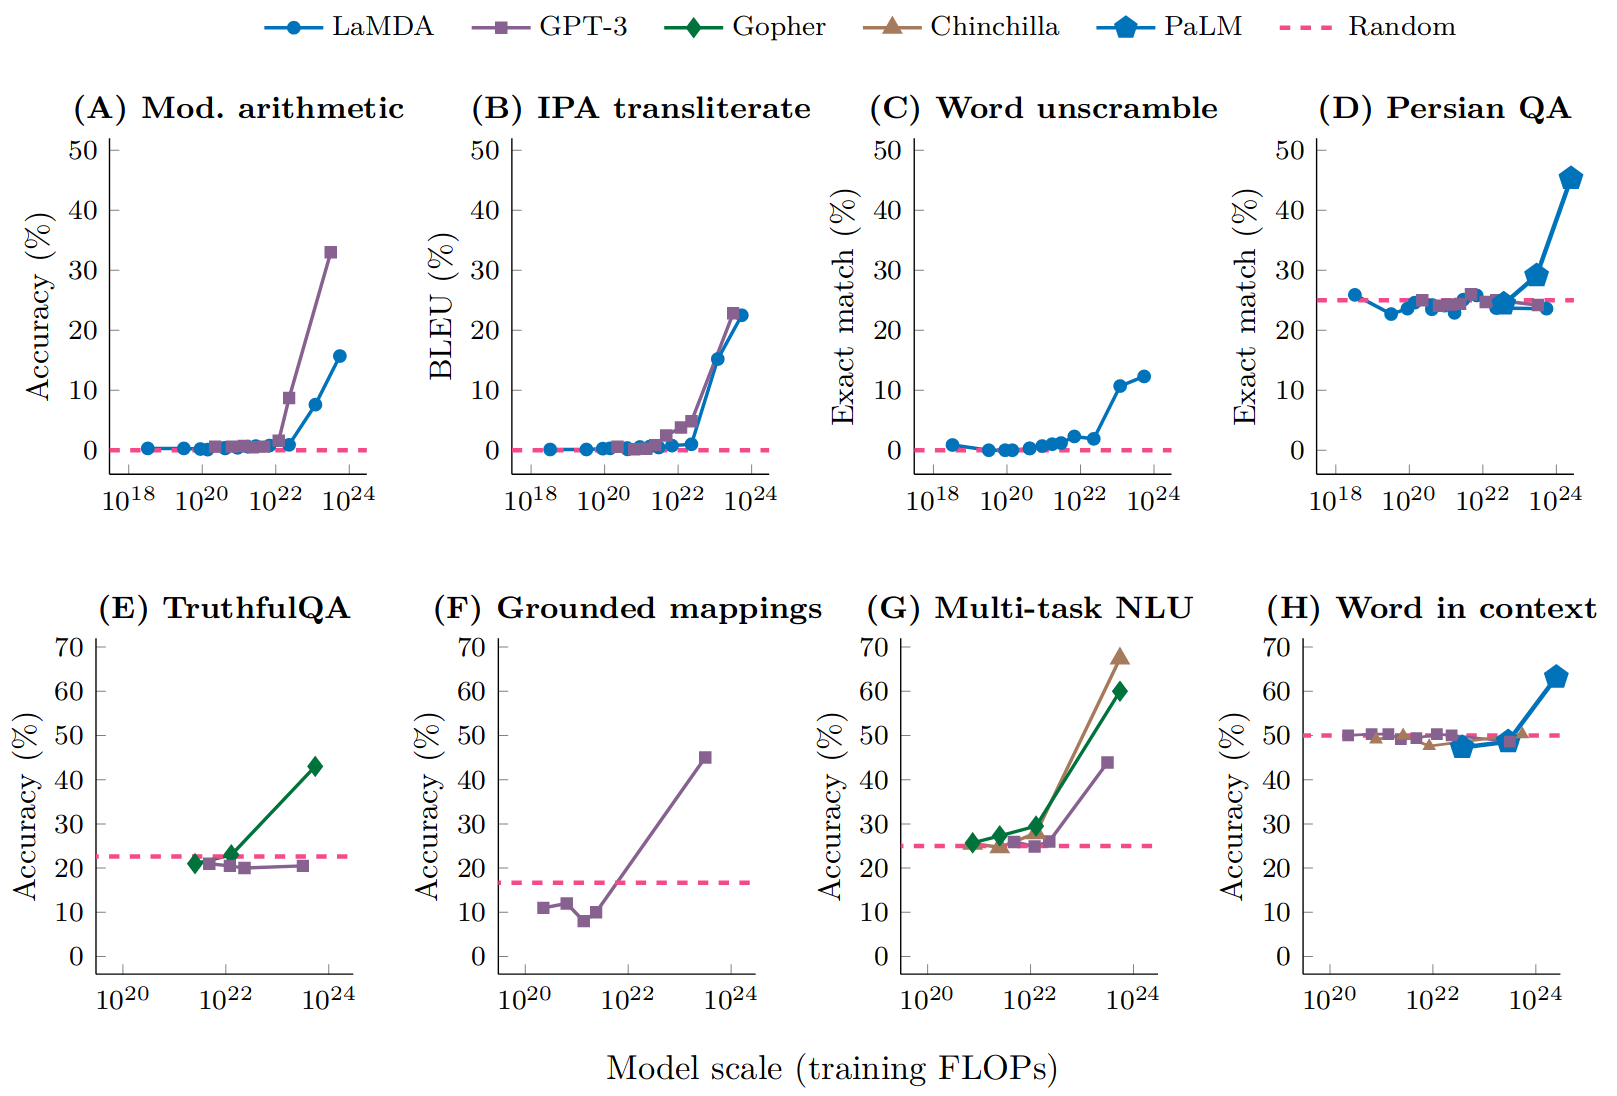
\includegraphics[width=0.9\textwidth]{figures/wei_2022_emergence/wei_2022_emergence_fig2.png}
    \caption{\textbf{Emergent abilities of large language models}. Model families display \textit{sharp} and \textit{unpredictable} increases in performance at specific tasks as scale increases.
    %Emergent abilities \cite{wei2022emergent} have also previously been labeled ``abrupt, specific capability scaling" \cite{ganguli2022predictability}, ``breakthrough capabilities" \cite{srivastava2022beyond} and ``sharp left turns" \cite{krakovna2022sharp1, krakovna2022sharp2}.
    Source: Fig. 2 from \cite{wei2022emergent}.}
    \label{fig:wei_2022_emergence_fig1}
\end{figure}

These emergent abilities have garnered significant interest, raising questions such as: What controls \textit{which} abilities will emerge?
What controls \textit{when} abilities will emerge? 
How can we make desirable abilities emerge faster, and ensure undesirable abilities never emerge? 
These questions are especially pertinent to AI safety and alignment, as emergent abilities forewarn that larger models might one day, without warning, acquire undesired mastery over dangerous capabilities \cite{steinhardt2022future,hendrycks2022emergent, krakovna2022sharp1, krakovna2022sharp2}.

In this paper, we call into question the claim that LLMs possess emergent abilities, by which we specifically mean \textit{sharp} and \textit{unpredictable} changes in model outputs as a function of model scale on specific tasks.
Our doubt stems from the observation that emergent abilities seem to appear only under metrics that nonlinearly or discontinuously scale any model's per-token error rate.
For instance, as we later show, $>92\%$ of emergent abilities on BIG-Bench tasks \cite{srivastava2022beyond} (hand-annotated by \cite{wei2022bigbench}) appear under either of these two metrics:
%
\begin{align*}
    \text{Multiple Choice Grade} \, &\defeq \, \begin{cases} 1 & \text{if highest probability mass on correct option} \\ 0 & \text{otherwise} \end{cases}\\
    \text{Exact String Match} \, &\defeq \, \begin{cases} 1 & \text{if output string exactly matches target string} \\ 0 & \text{otherwise} \end{cases}
    % \text{ROUGE-L-Sum} &= \text{See App. } \ref{app:metric_scaling:rougeLsum}\\
    % \text{BLEU} &= \text{See App. } \ref{app:metric_scaling:bleu}
\end{align*}

This raises the possibility of an alternative explanation for the origin of LLMs' emergent abilities: sharp and unpredictable changes might be induced by the researcher's choice of measurement, even though the model family's per-token error rate changes smoothly, continuously and predictably with increasing scale. 
Specifically, our alternative posits that emergent abilities are a mirage caused primarily by the researcher choosing a metric that nonlinearly or discontinuously deforms per-token error rates, and secondarily by possessing too few test data to accurately estimate the performance of smaller models, thereby causing smaller models to appear wholly unable to perform the task.
%and partially by evaluating too few large-scale models.

To communicate our alternative explanation, we present it as a simple mathematical model and demonstrate how it quantitatively reproduces the evidence offered in support of emergent abilities of LLMs. We then test our alternative explanation in three complementary ways:
%
\begin{enumerate}
    \item We make, test and confirm three predictions based on our alternative hypotheses using the InstructGPT \cite{lowe2022instruct} / GPT-3 \cite{brown2020language} model family.
    \item We meta-analyze published benchmarks \cite{srivastava2022beyond, wei2022emergent} to reveal that emergent abilities only appear for specific metrics, not for model families on particular tasks, and that changing the metric causes the emergence phenomenon to evaporate.
    \item We induce never-before-seen, seemingly emergent abilities in multiple architectures across various vision tasks by intentionally changing the metrics used for evaluation.
\end{enumerate}

